\documentclass[12pt, a4paper]{article}
\usepackage[utf8]{inputenc}
\usepackage{hyperref}
\usepackage[T1]{fontenc}
\usepackage{typearea}
\usepackage{scrpage2}
\usepackage{vmargin}
\usepackage{color}
\usepackage{fancyvrb}
\usepackage{listings}
\usepackage{graphicx}
\lstset{inputencoding=ansinew}
\usepackage{framed}
\usepackage{xcolor}
\usepackage[section]{placeins}
\usepackage{enumitem}
\setlist[enumerate,1]{start=0}
\hypersetup{
    colorlinks,
    linkcolor={red!50!black},
    citecolor={blue!50!black},
    urlcolor={blue!80!black}
}

\pagestyle{scrheadings}

\setpapersize{A4}
\setmargins{1.5cm}{1.5cm} % linker & oberer Rand
           {18cm}{25cm}   % Textbreite und -hoehe
           {12pt}{25pt}   % Kopfzeilenhoehe und -abstand
           {12pt}{30pt}   % \footheight (egal) und Fusszeilenabstand
\setlength{\headheight}{1.1\baselineskip}

\begin{document}

\part*{\begin{center}Digital Preservation\end{center}}
\begin{center}
Task 3: Documenting eScience experiments\\
Relationship between volcanoes and earthquakes\\

Arber Kryeziu, 0825135\\
Enri Miho, 0929003\\
Report
\end{center}

\section{Project application phase}
\subsection{Experiment overview and diagram}
Research has shown that the most usual earthquakes are caused through friction and sliding of tectonic plates one on top of the other\footnote{\url{http://pubs.usgs.gov/gip/dynamic/historical.html}}. Other factors may be ground instability (e.g. methane gas underground) and explosions. Moreover, since earthquakes and volcanoes usually occur near the edges of tectonic plates, it is known that volcanoes always cause quakes of different magnitudes due to the moving of lava to the surfacer\footnote{\url{https://pubs.usgs.gov/imap/2800/}}.\\
In this experiment, through parsing, analysing and visualizing the data collected by the renowned Smithsonian Institution's Global Volcanism Program (GVP)\footnote{\url{http://volcano.si.edu/gvp_about.cfm}} it will be demonstrated how many volcanic eruptions are placed within a given radius (should be at least 40 km) of an earthquake’s epicenter. Data about volcanoes consist of 10,000 years of Earth's volcanism, whereby data about earthquakes consist of only earthquakes with high Richter\footnote{\url{https://en.wikipedia.org/wiki/Richter_magnitude_scale}} magnitudes ( > 4)  from year 1964 - 2007.\\
All the parsed and analysed data will be visualized at the end. Moreover, some textual results will be extracted at the end of the experiment showing the number of volcanoes and earthquakes parsed, the relation of each volcano to the number of earthquakes as well as the correlation percentage (also labeled as dependency ratio) for a given volcano radius.\\
\newline
Figure 1 depicts the experiment. It consists of the following actions:
\begin{itemize}
\item {\bf Getting volcanoes.txt and earthquakes.txt:} First the script will try to connect to the database where these files are hosted and download them using \verb|wget|. If the connections fails for some reason, then the script will look if these files are locally available i.e were already downloaded (in any case, we provide the source files as backup). Right after this the java application will start.
\item {\bf Parsing volcanoes.txt and earthquakes.txt:} The volcanoes and earthquakes are parsed to entity objects to make further processing of the data easier.
\item {\bf Choosing the max volcano radius:} This is a very crucial step, the outcome will depend on this value. It represents the maximum distance a volcano and an earthquake's epicenter can have (in meters). If the distance is smaller than this value, then there is a correlation between the volcano and the earthquake, otherwise not. The default value in the script is \verb|40000m|. Note that this is still considered as a relatively small value for such a radius.
\item {\bf Checking for dependencies:} Now the program will check for every volcano if it depends on at least one of the earthquakes. This operation can be time consuming and will depend on the size of the data.
\item {\bf The result:} The program will generate than a result which will tell if there is a correlation between volcanoes and earthquakes or not. If the dependency ratio - this is the ratio of the number of volcanoes which depend on some earthquake and the overall number of the volcanoes - is greater or equal to 0.7, then there is a correlation, otherwise not.
\item {\bf The GUI:} The user interface will help visualizing the result of the experiment using Google Maps (using the google maps v3 api in javascript). The distribution of the volcanoes and the earthquakes can also be visualized. For preservation purposes, screenshots can be generated too. 
\end{itemize}
\begin{figure}[h]
  \centering
    \includegraphics[scale=0.15]{diagram}
    \caption{State diagram of the experiment}
\end{figure}

\subsection{Other publications}
The data used for this experiment are publicly available, free to use. Since they are relatively rich in content and capture a broad time span of tectonic occurrences, these data are the leading source for many of other publications and projects related to tectonic and volcanic activities\footnote{\url{http://ngdc.noaa.gov/hazard/volcano.shtml}}. However, through our research, we could not find experiments and analysis on all the data provided by our sources, as well as their relation to each other in the same approach as we do for this experiment. However, throughout the internet there are interactive maps which show only the latest seismic activities (i.e.. they include only a small subset of data from the same source we use)\footnote{Tilling, Robert I., et al. "This Dynamic Planet World Map of Volcanoes, Earthquakes, Impact Craters, and Plate Tectonics." (1994).}.


\section{Project execution phase}
\subsection{Experiment execution monitoring and execution model analysis}
After we developed our script for executing and starting the data visualization tool for the experiment, we installed and ran the data capture module of PMF (v1.0 beta) software as it is instructed in PMF website\footnote{\url{http://www.ifs.tuwien.ac.at/dp/process/projects/pmf.html}}. Workflow execution monitoring did run without any issues in a Linux Virtual Machine. The whole process did not take more than three minutes. Below is the exact command used for capturing:
\begin{lstlisting}[breaklines]
sudo java -jar capture-1.0-SNAPSHOT.jar -a /home/enrimilan/Desktop/dp-experiment/scripts/experiment.sh -d  /home/enrimilan/Desktop/capture
\end{lstlisting}
The (zipped) extract generated from PMF (\verb|data.zip|), was used in the execution model analysis phase. More specific, we imported the \verb|data/process.owl|  ontology file into Protégé (v.5.0.0)\footnote{\url{http://protege.stanford.edu/products.php}}.  We browsed throughout the individuals of the ontology which captured the actual data of the processes executed.\\
Finally, we started experimenting and writing SPARQL queries to easily retrieve results from the actual captured data (see the queries in SPARQL.txt). The results of each query:
\begin{enumerate}
\item Display identifier and user of the system for which the execution was captured.\\
\newline
\noindent\fbox{%
    \parbox{\textwidth}{%
        {\bf identifier:} xrn://+machine?+hostid=007f0101/+hostname=ubuntu\\
        {\bf user:} root
    }%
}

\item Display version of the operating system\\
\newline
\noindent\fbox{%
    \parbox{\textwidth}{%
        {\bf os:} ‘Ubuntu 16.04 LTS’
    }%
}\\
\newline
{\bf Note:} Data capturing has been conducted in a linux virtual machine

\item List Debian packages that are need by the experiment for execution\\
\newline
\noindent\fbox{%
    \parbox{\textwidth}{%
        {\bf packages:}\\
        libuuid1	
openjdk8jreheadless	
libkrb526heimdal	
libheimbase1heimdal	
libp11kit0	
basefiles	
libkeyutils1	
libc6	
locales	
libhogweed4	
libnettle6
libldap242	
libgssapikrb52	
libgmp10	
wget	
libroken18heimdal
libtinfo5	
libidn11	
libsqlite30	
libtasn16	
libheimntlm0heimdal	
libkrb5support0	
libcurl3gnutls	
libk5crypto3	
libgnutls30	
libkrb53	
libhx5095heimdal	
curl	
libasn18heimdal	
libpcre3	
libc6dbg	
libssl100	
libcomerr2	
libgssapi3heimdal	
libnssmdns	
libsasl22	
libffi6	
libhcrypto4heimdal	
libwind0heimdal	
librtmp1	
zlib1g
        
    }%
}

\item List data files read and written by the experiment (hint: check System Software)\\
\newline
\noindent\fbox{%
    \parbox{\textwidth}{%
        {\bf data\_files:}\\
        /usr/lib/locale/locale-archive\\
/home/enrimilan/.wget-hsts\\
/home/enrimilan/Downloads/pmf-1.0/capture/volcanoes.txt\\
/home/enrimilan/Downloads/pmf-1.0/capture/earthquakes.txt\\
/home/enrimilan/Desktop/dp-experiment/scripts/\\
/home/enrimilan/Desktop/dp-experiment/scripts/experiment.sh\\
    }%
}\\
\newline
{\bf Note:} These are the only data captured. A manual look in Protege into the  ‘System Service’ shows only the last entry from the above list (i.e. \verb|experiment.sh|). 

\item Check whether the processes communicates with external services (ASK query)\\
\newline
\noindent\fbox{%
    \parbox{\textwidth}{%
        {\bf True \\ False}
        
    }%
}\\
\newline
{\bf Note:} The experiment uses only HTTP service to download the source data and another HTTP service to render the results of experiment (see note in next query)

\item List addresses of external services\\
\newline
\noindent\fbox{%
    \parbox{\textwidth}{%
       {\bf services:}\\
127.0.1.1\\
160.111.244.21
    }%
}\\
\newline
{\bf Note:} The first IP address is the localhost (experiment was conducted in a Linux Virtual Machine). The second one is the IP address of the ‘Smithsonian Institute’ server, from which source files (volcanoes.txt and earthquakes.txt) are downloaded. However, our analysis tool (Experiment.jar) uses also Google Maps API (v.3) to render the result. The service address was not captured and was nowhere to be found in owl file.

\item List dependencies that are neither data files, nor Debian packages, but are still used in the experiment.\\
\newline
\noindent\fbox{%
    \parbox{\textwidth}{%
       {\bf dependencies:}\\
`Process\_0, /home/enrimilan/Desktop/dp-experiment/scripts/experiment.sh	\\
‘Process\_1, /usr/bin/curl\\
‘process\_3, /usr/bin/wget\\	
‘process\_4, /usr/bin/curl\\
‘process\_6, /usr/bin/wget\\
‘process\_7, /usr/bin/java
    }%
}\\
\newline
{\bf Note:} These are the dependencies used when executing the script. The script itself uses ‘curl’ and ‘wget’ to fetch the server and download source data. This is done two times, one time for the volcanoes list, and the other time for the earthquakes list. Afterwards our data analysis tool (.jar) is started using ‘java’ by the script.

\end{enumerate}

\subsection{Data characterisation}
All the files used and produced by executing our experiment (see result of SPARQL query 3) were imported in DROID\footnote{\url{http://digital-preservation.github.io/droid/}} to identify their format as well as extract other features. A report of each file was generated and exported in CSV file (see accompanied file \verb|RelationshipVolcanousEarthquakes.csv|). Moreover, we extracted the size and mime-types of files and used excel sheets to aggregate and visualize results (see figure 2).
\begin{figure}[h]
  \centering
    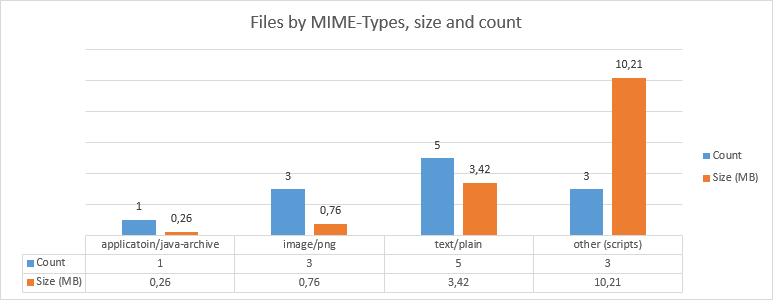
\includegraphics[scale=0.85]{graph}
    \caption{The total number of files used and generated through the experiment is {\bf 12} with a sum size of {\bf 14,66 MB}.}
\end{figure}

\subsection{Validation requirements}
The validation requirements can be seen in table 1.
\begin{table}[h]
\centering
\begin{tabular}{|p{0.5cm}|p{3.0cm}|p{3.5cm}|p{3.0cm}|p{1.5cm}|p{3.0cm}|p{2.0cm}|}
\hline
 \textbf{ID} & \textbf{Requirement} & \textbf{Sub-requirement} & \textbf{Metric} & \textbf{Target value} & \textbf{Measurement point} & \textbf{Tool} \\ \hline
 R1 & Experiment results must be identical for a given earthquake perimeter (default 40km) & Source files must have same number of entries as those provided as backup & 
Correlation factor 0.7 (i.e. 70\%) that a vulcan center point is within the given radius of an earthquake epicenter
 & 0 deviation on correlation percentage & Correlation percentage exported (in results.txt) & Correlation percentage exported (in results.txt) \\ \hline
 R2 &  Source files should have same format as those provided by us (volcanoes.txt , earthquakes.txt) & Plain Text Files (txt) & &
All entries should have same formating structure & Tabulated formating structure & Data analysis (parsing inside Experiment.jar)      \\ \hline
\end{tabular}
\caption{Validation requirements}
\end{table}

\subsection{Data Management Plan (DMP)}

\subsection{Data sharing}
The sources can be found at \url{https://github.com/enrimilan/dp-experiment}

\end{document}